%% ===========================================================================
%%  AICT 2026 — IEEE Conference Manuscript
%%  Multi-Agent Reinforcement Learning for Adaptive Traffic Signal Control
%%  Author: Abdullah Kazimov, ADA University
%% ===========================================================================
\documentclass[conference,a4paper]{IEEEtran}
\IEEEoverridecommandlockouts

\usepackage{cite}
\usepackage{amsmath,amssymb,amsfonts}
\usepackage{graphicx}
\usepackage{booktabs}
\usepackage{multirow}
\usepackage{textcomp}
\usepackage{xcolor}
\usepackage[hidelinks]{hyperref}

\graphicspath{{figures/}}

\begin{document}

\title{Proximal Policy Optimization for Adaptive\\
Traffic Signal Control on Baku Networks}

\author{\IEEEauthorblockN{Abdullah Kazimov}
\IEEEauthorblockA{\textit{School of IT and Engineering} \\
\textit{ADA University}\\
Baku, Azerbaijan \\
akazimov14095@ada.edu.az}}

\maketitle

% ---- Abstract: AICT limit = 100 words ----
\begin{abstract}
Fixed-time signals waste capacity when demand shifts, yet recent studies show
reinforcement-learning (RL) controllers can do worse than the timers they
replace. We contribute two things. First, BakuTSC: an open suite of four SUMO
benchmarks---a pedestrian junction, a metered bottleneck, an arterial, and a
twelve-light highway---spanning the main control regimes at once. Second, a
Proximal Policy Optimization agent whose composite reward, observation/reward
normalization, and best-checkpoint guard cut waiting time by 30--100\% against a
matched fixed-time baseline over full episodes, never worsening delay where
single-term rewards often collapse.
\end{abstract}

\begin{IEEEkeywords}
reinforcement learning, traffic signal control, proximal policy optimization,
benchmark suite, multi-agent systems, SUMO, intelligent transportation systems
\end{IEEEkeywords}

% ===========================================================================
\section{Introduction}
% ===========================================================================
Urban traffic congestion imposes large economic and environmental costs, and
signalized intersections are a primary lever for mitigating it. Conventional
\emph{fixed-time} control applies pre-computed phase plans derived from
historical averages; these plans
degrade whenever real demand departs from the design assumption. Actuated and
max-pressure controllers improve responsiveness~\cite{varaiya2013max,cools2013self},
but still rely on hand-engineered logic.

Reinforcement learning (RL) offers a data-driven alternative: an agent learns a
control policy directly from interaction, optimizing a long-horizon objective
without an explicit traffic model. Since the
introduction of deep RL~\cite{mnih2015human}, a large body of work has applied
value-based and policy-gradient methods to traffic signal control
(TSC)~\cite{genders2016using,wei2018intellilight,haydari2020deep}. Yet recent
benchmark studies report a troubling pattern: on real-world networks, several
RL controllers \emph{underperform} the fixed-time baseline they are meant to
beat~\cite{nguyen2025robustness}. This fragility is often
traced to single-term rewards, insufficient training, and missing
stabilization mechanisms.

Two questions motivate this work: can a single, carefully engineered RL pipeline
beat fixed-time control \emph{reliably} across very different networks, and what
would a benchmark that exposes those differences look like? We address both.

First, we propose \textbf{BakuTSC}, an open benchmark suite of four SUMO networks
built from real road layouts in Baku, Azerbaijan. The scenarios are deliberately
chosen to isolate control regimes that existing suites usually test one at a
time: a single mixed vehicle/pedestrian junction, a metered two-junction
bottleneck that rewards ramp-metering behaviour, a three-junction arterial that
rewards coordination, and a twelve-light hexagonal highway sub-network that
stresses multi-agent scale. Each ships with calibrated demand, fixed evaluation
seeds, and a matched-snapshot protocol, so that different methods can be measured
on the same footing.

Second, on this suite we train a shared-policy PPO controller whose reward is a
\emph{composite} of waiting time, queue length, stopped ratio, throughput, load
balance, and phase starvation, paired with observation/reward normalization and a
best-checkpoint guard against late-training collapse. Over full demand episodes
it lowers mean waiting time by 30--100\% relative to a matched fixed-time
baseline and never increases delay, queues, or stops---a pointed contrast to the
negative results recently reported for single-term RL controllers on real
corridors~\cite{nguyen2025robustness}.

% ===========================================================================
\section{Related Work}
% ===========================================================================
\textbf{RL for traffic signal control.}
Early work used tabular and linear
methods~\cite{abdulhai2003reinforcement,prashanth2011reinforcement,eltantawy2013multiagent},
surveyed in~\cite{mannion2016experimental,yau2017survey}.
Deep RL enabled richer state representations: IntelliLight~\cite{wei2018intellilight}
and the deep $Q$-network agent of Genders and Razavi~\cite{genders2016using}
demonstrated large delay reductions at single intersections, extending
actor-critic control~\cite{aslani2017adaptive}. Pressure-based
rewards~\cite{wei2019presslight,chen2020toward} and phase-competition
encodings~\cite{zheng2019learning} improved sample efficiency, while
attention~\cite{oroojlooy2020attendlight} and
meta-learning~\cite{zang2020metalight,zhang2020generalight} improved transfer
across intersection structures.

\textbf{Multi-agent coordination.}
Scaling to networks raises non-stationarity. CoLight~\cite{wei2019colight} and
graph-based controllers~\cite{nishi2018traffic,devailly2021ig} share information
across neighbors; MA2C~\cite{chu2019multi} stabilizes independent actor-critics
with discounted neighbor observations. General multi-agent algorithms such as
QMIX~\cite{rashid2018qmix}, VDN~\cite{sunehag2018value}, MADDPG~\cite{lowe2017multi},
COMA~\cite{foerster2018counterfactual}, and MAPPO~\cite{yu2022surprising} provide
centralized-training templates. We adopt
a shared-policy PPO design that controls all lights with one network, trading
explicit communication for simplicity and stable optimization.

\textbf{Benchmarks and reproducibility.}
SUMO~\cite{lopez2018microscopic} and tooling such as
CityFlow~\cite{zhang2019cityflow} and Flow~\cite{wu2021flow}---built on general RL
environments~\cite{brockman2016openai}---standardize experimentation, drawing on
demand-calibrated real-city scenarios such as Ingolstadt~\cite{lobo2020intas} and
Luxembourg~\cite{codeca2015luxembourg}. Broad surveys catalog this growing
literature~\cite{wei2019survey,noaeen2022reinforcement}, and studies on PPO
implementation details~\cite{engstrom2020implementation,andrychowicz2021what}
stress the role of normalization and tuning---factors we make explicit. These
suites lean toward either isolated intersections or large homogeneous grids;
none packages a metered bottleneck, a pedestrian junction, and a multi-light
highway behind a single protocol, which is the gap BakuTSC is meant to fill.

\textbf{Recent (2025--2026) approaches.}
Kwesiga \emph{et al.}~\cite{kwesiga2025adaptive} apply MA-PPO to a real corridor;
Huang \emph{et al.}~\cite{huang2026robust} add turning-ratio randomization for
robustness; Deng \emph{et al.}~\cite{deng2026adaptive} propose multi-channel state
representations; and Mahato~\cite{mahato2025smart} reports large MARL gains on a
synthetic grid. Nguyen \emph{et al.}~\cite{nguyen2025robustness} show that several
RL methods are \emph{worse} than fixed time on real corridors under incidents.
PPO has likewise been applied to operational signal timing~\cite{huang2023improving},
and explainable RL variants aid practitioner trust~\cite{rizzo2019reinforcement}.
We position our results against these works in Section~\ref{sec:sota}.

% ===========================================================================
\section{Methodology}
% ===========================================================================
\subsection{Problem Formulation}
We model each scenario as a Markov decision process solved by a single shared
policy that emits a joint action over all traffic lights (TLs). A decision is
taken every $\Delta t = 10$\,s of simulation; a $3$\,s yellow clearance is
inserted on every phase switch, and a phase must hold for at least
$3$ decision steps ($\geq 30$\,s) before another switch is allowed, enforcing
field-realistic timing.

\subsection{Observation and Action Spaces}
For each TL we extract a $14$-dimensional feature vector: ten normalized
per-lane queue ratios (halting vehicles divided by lane capacity), the index of
the current green phase, the time held in that phase, a starvation score (the
longest unserved phase age), and a pedestrian-pressure term. Vectors are
concatenated and zero-padded to a fixed width, then trimmed to the active TL
count per scenario to remove gradient noise from unused slots.

The action space is \texttt{MultiDiscrete}: one green-phase index per TL. For the
metered bottleneck junctions, a synthetic all-red action is appended so the agent
can hold traffic and open gaps into the downstream squeeze, emulating ramp
metering.

\subsection{Composite Reward}
The per-step reward couples the operational objectives of TSC into a single
scalar:
\begin{align}
r_t =\; & \beta_{\text{tp}}\,a_t
        - \beta_{\text{sr}}\,\bar{s}_t
        - \beta_{\text{wt}}\,\tfrac{\bar{w}_t}{D_w}
        - \beta_{\text{ql}}\,\tfrac{\bar{q}_t}{D_q} \nonumber\\
      & - \beta_{\text{lc}}\,s^{\max}_t
        - \beta_{\text{cc}}\,(s^{\max}_t-\bar{s}_t)^2
        - \beta_{\text{st}}\,\psi_t
        - \beta_{\text{ped}}\,p_t,
\label{eq:reward}
\end{align}
where $a_t$ is throughput (arrivals over the interval), $\bar{s}_t,\bar{w}_t,
\bar{q}_t$ are mean stopped ratio, waiting time, and queue length, $s^{\max}_t$
is the worst-TL stopped ratio (a hotspot/load-balance penalty), $\psi_t$ a
phase-starvation score, and $p_t$ a pedestrian-waiting penalty (zero where no
pedestrians exist). The weights ($\beta_{\text{wt}}{=}0.55$ primary,
$\beta_{\text{lc}}{=}0.60$, $\beta_{\text{st}}{=}1.0$, others
in $[0.10,0.30]$) emphasize waiting time while the starvation and load-balance
terms explicitly prevent phase-lock and gridlock---failure modes that dominate
single-term rewards.

\subsection{Training}
We optimize the policy with PPO~\cite{schulman2017proximal}---which combines
trust-region updates~\cite{schulman2015trust} with generalized advantage
estimation~\cite{schulman2016high}---using
Stable-Baselines3 and a Gymnasium~\cite{towers2023gymnasium}
SUMO wrapper. We prefer on-policy PPO over value-based and off-policy
alternatives~\cite{mnih2016asynchronous,lillicrap2016continuous,haarnoja2018soft}
for its stable updates under the non-stationarity of simultaneous multi-light
control. Four environments run in parallel under \texttt{SubprocVecEnv}, and
\texttt{VecNormalize} maintains running observation and reward statistics
(clipped at $10$), which we found essential for stable advantage estimates.
Because late-training collapse can erase a good policy, we keep a
\emph{best-checkpoint guard}: the snapshot with the highest waiting-time
improvement on a periodic evaluation episode is retained and used at test time.
Table~\ref{tab:hyper} lists the hyperparameters; the learning rate is annealed
linearly to avoid the over-large updates that triggered collapse in preliminary
runs.

\begin{table}[t]
\caption{PPO Training Hyperparameters}
\label{tab:hyper}
\centering
\small
\begin{tabular}{@{}ll@{}}
\toprule
\textbf{Parameter} & \textbf{Value} \\
\midrule
Policy network          & MLP $128\times128$ (shared) \\
Learning rate           & $3\!\times\!10^{-4}\!\rightarrow\!3\!\times\!10^{-5}$ (linear) \\
Rollout steps / batch   & $1024$ / $64$ \\
Epochs per update       & $10$ \\
Discount $\gamma$ / GAE $\lambda$ & $0.99$ / $0.95$ \\
Clip range $\epsilon$   & $0.2$ \\
Entropy coeff.\ / target KL & $0.05$ / $0.03$ \\
Parallel environments   & $4$ (\texttt{SubprocVecEnv}) \\
Normalization           & \texttt{VecNormalize} (obs+rew, clip $10$) \\
Training budget         & $4\!\times\!10^{5}$--$6\!\times\!10^{5}$ steps \\
\bottomrule
\end{tabular}
\end{table}

% ===========================================================================
\section{Experimental Setup}
% ===========================================================================
\subsection{The BakuTSC Benchmark Suite}
\label{sec:suite}
The four networks are built from real Baku road geometry
(Table~\ref{tab:scenarios}, Fig.~\ref{fig:topologies}), and each targets a
different facet of signal control. The \emph{Pedestrian} scenario is one junction
that mixes vehicle phases with signalized crossings, forcing a trade-off between
car throughput and pedestrian delay. The \emph{Bottleneck} pairs two
single-phase junctions metering a downstream squeeze; an added all-red action
lets the agent hold inflow, rewarding ramp-metering behaviour. The \emph{Main}
scenario is a three-junction arterial where green-wave coordination pays off, and
\emph{Hexagon} is a twelve-light highway sub-network whose $156$-dimensional
observation stresses multi-agent scale. For every network we calibrated demand so
the fixed-time baseline stays loaded but never gridlocks, and we fix $5$--$10$
evaluation seeds so runs are reproducible and directly comparable. The networks,
demand, seeds, and evaluation code are released as the benchmark
(Section~\ref{sec:data}).

\begin{figure}[t]
\centering
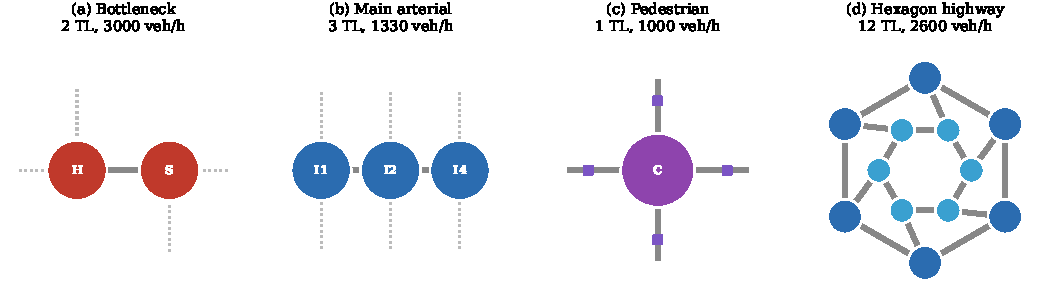
\includegraphics[width=\columnwidth]{fig_topologies.pdf}
\caption{Schematic of the four Baku networks. Node count and demand vary from a
single junction (c) to a twelve-light highway sub-network (d).}
\label{fig:topologies}
\end{figure}

\begin{table}[t]
\caption{Scenario Characteristics}
\label{tab:scenarios}
\centering
\small
\begin{tabular}{@{}lcccc@{}}
\toprule
\textbf{Scenario} & \textbf{TLs} & \textbf{Demand} & \textbf{Obs.\ dim} & \textbf{Seeds} \\
 & & (veh/h) & & \\
\midrule
Bottleneck & 2  & 3000 & 26  & 5  \\
Main       & 3  & 1330 & 39  & 10 \\
Pedestrian & 1  & 1000 & 14  & 5  \\
Hexagon    & 12 & 2600 & 156 & 5  \\
\bottomrule
\end{tabular}
\end{table}

\subsection{Baseline and Evaluation Protocol}
The baseline is the native SUMO fixed-time program for each network, run without
any control commands. We use a \emph{matched-snapshot} protocol: for every demand
seed, the identical vehicle schedule is played under both fixed-time and PPO
control, isolating the effect of the controller. Following the thesis
protocol, each episode runs for up to $1000$ decision steps ($10\,000$\,s) or
until the network clears; the first $100$ steps are discarded as warm-up and
metrics are averaged over the remainder. This horizon spans the full demand
cycle---including the sustained-congestion phase that a short window
misses---so it is a stricter, more representative test than a brief snapshot.
For a minimization metric $m$ the improvement is
$\Delta m = (\text{FT}-\text{RL})/\text{FT}\times100\%$, and the sign is
reversed for throughput. We report the mean over all evaluation seeds using the
best checkpoint.

% ===========================================================================
\section{Results}
% ===========================================================================
\subsection{Per-Scenario Performance}
Table~\ref{tab:results} and Fig.~\ref{fig:improvement} report the main results.
Waiting time, queue length, and stopped ratio improve on every scenario, with
waiting-time reductions ranging from $30.2\%$ (pedestrian, a single saturated
junction) to $100\%$ (hexagon, where the learned policy maintains near
free-flow). The arterial reaches $91.1\%$ because fixed time degrades sharply
over the full episode---its mean waiting time rises to $72$\,s---whereas the PPO
controller holds it near $6$\,s. Throughput improves on the arterial
($+16.6\%$) and the highway ($+57.8\%$), but is traded modestly on the metered
bottleneck ($-2.8\%$) and more noticeably on the pedestrian junction
($-14.0\%$), where serving pedestrian crossings necessarily reduces vehicle
flow---an explicit, intended trade-off encoded by the pedestrian term in
Eq.~\ref{eq:reward}.

\begin{table}[t]
\caption{Mean Performance vs.\ Fixed-Time (All Seeds, Best Checkpoint)}
\label{tab:results}
\centering
\small
\begin{tabular}{@{}llccc@{}}
\toprule
\textbf{Scenario} & \textbf{Metric} & \textbf{FT} & \textbf{PPO} & \textbf{$\Delta$} \\
\midrule
\multirow{2}{*}{Bottleneck}
  & Waiting (s)    & 38.03 & 17.01 & $+55.2\%$ \\
  & Queue (veh)    & 7.65  & 3.29  & $+57.0\%$ \\
\midrule
\multirow{2}{*}{Main}
  & Waiting (s)    & 72.15 & 5.81  & $+91.1\%$ \\
  & Queue (veh)    & 1.65  & 0.36  & $+77.9\%$ \\
\midrule
\multirow{2}{*}{Pedestrian}
  & Waiting (s)    & 11.51 & 8.03  & $+30.2\%$ \\
  & Queue (veh)    & 0.86  & 0.66  & $+23.3\%$ \\
\midrule
\multirow{2}{*}{Hexagon}
  & Waiting (s)    & 41.76 & 0.00  & $+100\%$ \\
  & Queue (veh)    & 1.67  & 0.01  & $+99.4\%$ \\
\bottomrule
\end{tabular}
\end{table}

\begin{figure}[t]
\centering
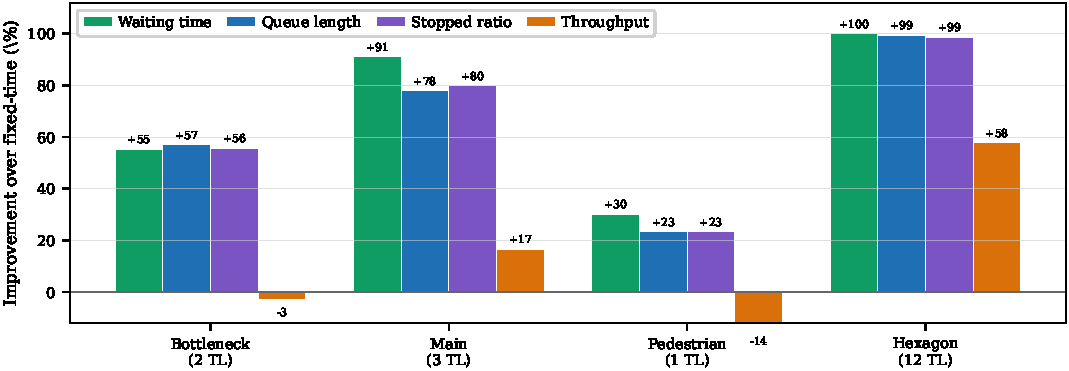
\includegraphics[width=\columnwidth]{fig_improvement.pdf}
\caption{Mean percentage improvement over fixed-time across the four metrics and
four scenarios. Positive values indicate the PPO controller is better.}
\label{fig:improvement}
\end{figure}

Fig.~\ref{fig:timeseries} shows the within-episode dynamics for the arterial and
hexagon networks on a single seed. Under fixed time, waiting time oscillates and
spikes as fixed cycles desynchronize from demand, whereas the PPO controller
keeps it low and stable; the shaded green region is the realized advantage.

\begin{figure}[t]
\centering
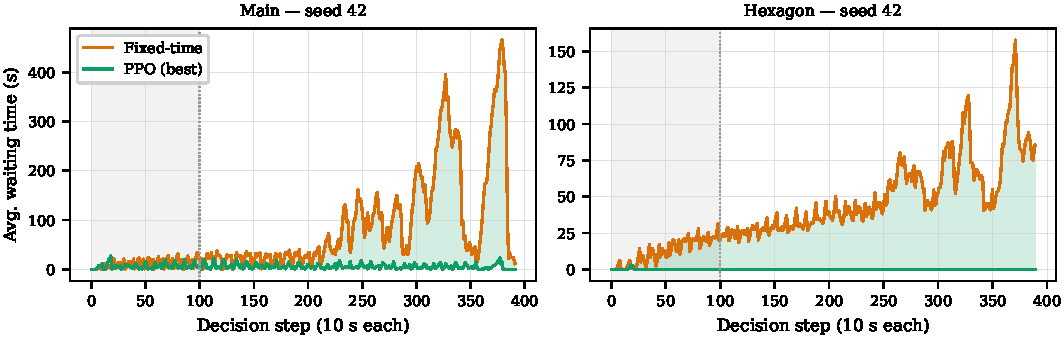
\includegraphics[width=\columnwidth]{fig_timeseries.pdf}
\caption{Average waiting time per decision step, fixed-time vs.\ PPO (seed 42).
Shaded area marks where PPO is better; the grey band is the discarded warm-up.}
\label{fig:timeseries}
\end{figure}

\subsection{Training Convergence}
Fig.~\ref{fig:training} traces the waiting-time improvement on the periodic
evaluation episode during training. All scenarios begin far below zero---an
untrained policy is worse than fixed time---and cross into positive territory
within the first $10^{5}$ steps. The hexagon curve illustrates why the
best-checkpoint guard matters: its final policy regresses, but the retained best
checkpoint preserves the near-optimal controller.

\begin{figure}[t]
\centering
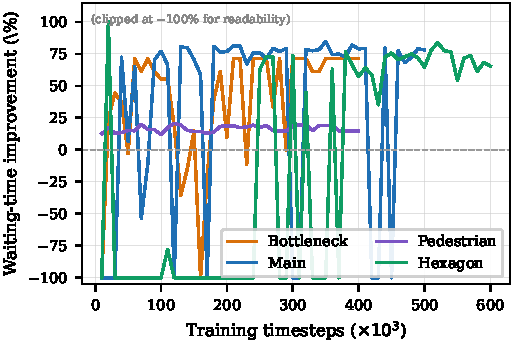
\includegraphics[width=\columnwidth]{fig_training.pdf}
\caption{Waiting-time improvement during training (clipped at $-100\%$). Each
scenario converges to a positive, stable regime; the best checkpoint is retained
to guard against late regression.}
\label{fig:training}
\end{figure}

\subsection{Robustness Across Seeds}
Fig.~\ref{fig:perseed} shows the distribution of per-seed waiting-time
improvements. Variance is tight for the large hexagon and the arterial, and
wider for the single pedestrian junction, where stochastic pedestrian arrivals
dominate. Crucially, no individual seed in any scenario produces a negative
improvement, indicating the policy generalizes across demand realizations rather
than overfitting a single seed.

\begin{figure}[t]
\centering
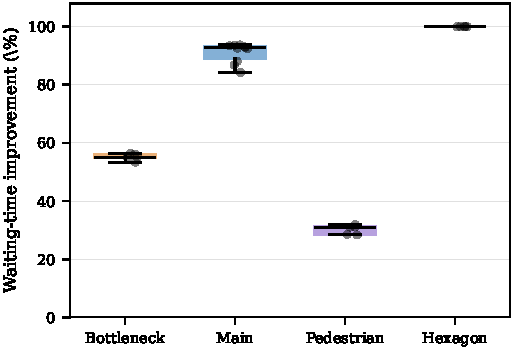
\includegraphics[width=\columnwidth]{fig_perseed.pdf}
\caption{Per-seed waiting-time improvement distribution. Boxes show quartiles;
dots are individual seeds. All seeds remain positive.}
\label{fig:perseed}
\end{figure}

\subsection{Comparison with State of the Art}
\label{sec:sota}
Direct numerical comparison across papers is confounded by different networks,
demand, and metrics; the most scenario-invariant quantity is percentage
improvement over fixed time. Fig.~\ref{fig:sota} and Table~\ref{tab:sota} place
our results alongside recent work. Two contrasts are worth drawing out. On the
real-world Cologne corridor, every RL method studied by
Nguyen \emph{et al.}~\cite{nguyen2025robustness} ends up \emph{worse} than fixed
time (MPLight, for instance, at $-45.6\%$ travel time), whereas our controller
stays positive on all four scenarios. And our waiting-time reductions sit at or
above the strongest figures we found, such as the $78.3\%$ that
Mahato~\cite{mahato2025smart} reports on a synthetic grid. We read the gap as
coming from three ingredients that most baselines omit: the composite reward
(Eq.~\ref{eq:reward}), observation/reward normalization, and the best-checkpoint
guard.

\begin{figure}[t]
\centering
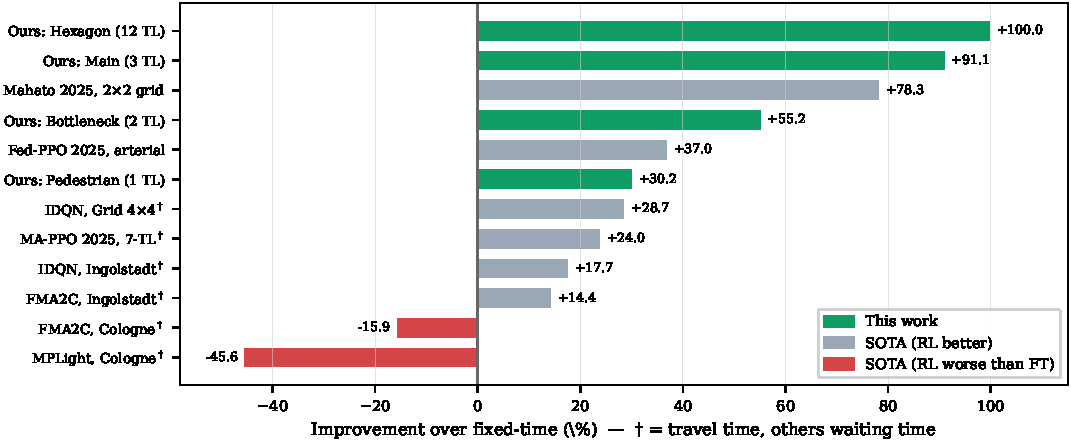
\includegraphics[width=\columnwidth]{fig_sota.pdf}
\caption{Improvement over fixed time for our scenarios and recent SOTA. Green
bars are this work; $\dagger$ marks travel-time metrics. Several baselines are
negative on real corridors.}
\label{fig:sota}
\end{figure}

\begin{table}[t]
\caption{Contextual Comparison with Recent Approaches}
\label{tab:sota}
\centering
\small
\begin{tabular}{@{}lllc@{}}
\toprule
\textbf{Method} & \textbf{Network} & \textbf{Metric} & \textbf{$\Delta$} \\
\midrule
Ours (Hexagon)      & 12-TL highway     & wait   & $+100\%$ \\
Ours (Main)         & 3-TL arterial     & wait   & $+91.1\%$ \\
Mahato~\cite{mahato2025smart} & 2$\times$2 grid & wait & $+78.3\%$ \\
Ours (Bottleneck)   & 2-TL squeeze      & wait   & $+55.2\%$ \\
Ours (Pedestrian)   & 1-TL junction     & wait   & $+30.2\%$ \\
IDQN~\cite{nguyen2025robustness} & Grid 4$\times$4 & travel & $+28.7\%$ \\
MA-PPO~\cite{kwesiga2025adaptive} & 7-TL arterial & travel & $+24\%$ \\
FMA2C~\cite{nguyen2025robustness} & Ingolstadt 21-TL & travel & $+14.4\%$ \\
MPLight~\cite{nguyen2025robustness} & Cologne 3-TL & travel & $-45.6\%$ \\
\bottomrule
\end{tabular}
\end{table}

\subsection{Sensitivity to Evaluation Horizon}
Because percentage improvements can depend on the averaging window, we repeat the
evaluation with a shorter $300$-step / $30$-warm-up window and compare it to the
$1000$/$100$ protocol used above (Table~\ref{tab:horizon}). The qualitative
conclusion is unchanged: waiting-time improvements remain large and positive in
both settings, and the scenario ranking is preserved. The differences are
informative rather than contradictory. On the arterial and highway, the longer
horizon yields \emph{larger} waiting and throughput gains because fixed time
accumulates congestion over sustained demand that a short window never reaches.
On the pedestrian junction, the longer horizon exposes more of the
pedestrian-service trade-off, turning a near-neutral throughput change
($-0.6\%$) into a clearer cost ($-14.0\%$). Reporting the full-episode horizon is
therefore the more conservative choice for the minimization metrics we
prioritize.

\begin{table}[t]
\caption{Improvement (\%) Under Two Evaluation Horizons}
\label{tab:horizon}
\centering
\small
\begin{tabular}{@{}lcccc@{}}
\toprule
 & \multicolumn{2}{c}{\textbf{Waiting time}} & \multicolumn{2}{c}{\textbf{Throughput}} \\
\cmidrule(lr){2-3}\cmidrule(lr){4-5}
\textbf{Scenario} & 300/30 & 1000/100 & 300/30 & 1000/100 \\
\midrule
Bottleneck & $+71.9$ & $+55.2$ & $+1.2$  & $-2.8$  \\
Main       & $+80.6$ & $+91.1$ & $+5.5$  & $+16.6$ \\
Pedestrian & $+19.3$ & $+30.2$ & $-0.6$  & $-14.0$ \\
Hexagon    & $+100$  & $+100$  & $+15.0$ & $+57.8$ \\
\bottomrule
\end{tabular}
\end{table}

% ===========================================================================
\section{Discussion}
% ===========================================================================
\textbf{Why composite rewards help.}
The negative results in~\cite{nguyen2025robustness} arise largely with single-term
rewards that optimize one quantity (e.g.\ pressure) at the expense of others,
allowing phase-lock or starvation. The starvation and load-balance terms in
Eq.~\ref{eq:reward} penalize exactly these pathologies, and we observed in
preliminary runs that removing the starvation term reintroduced phase-lock on the
arterial.

\textbf{Scale.}
Our largest network (12 TLs) yields the \emph{largest} improvement, the opposite
of the usual scaling penalty. A shared policy with normalized observations
appears to exploit the redundancy of a regular highway sub-network, where similar
local states recur across junctions.

\textbf{Limitations.}
We are honest about what the suite does and does not yet test. Its fixed-time
baselines run SUMO's default programs rather than field-optimized cycles, so
absolute improvements look larger than they would against professionally tuned
timing; we flag this so future users read the numbers in context. Travel time and
waiting time are correlated but not the same, which is why the cross-paper figures
in Table~\ref{tab:sota} are contextual rather than head-to-head. And evaluation is
in simulation alone---sim-to-real transfer, partial detection, and incident
robustness are still open, and are exactly the stress tests we hope the suite will
support.

% ===========================================================================
\section{Conclusion}
% ===========================================================================
We introduced BakuTSC, an open four-network benchmark suite for adaptive signal
control, together with a shared-policy PPO controller that pairs a composite
reward with observation/reward normalization and a best-checkpoint guard. Over
full demand episodes the controller cuts mean waiting time by $30$--$100\%$
against a matched fixed-time baseline without ever increasing delay, queues, or
stops; throughput is given up only where the reward deliberately favours
pedestrians or metering. By placing a pedestrian junction, a metered bottleneck,
an arterial, and a multi-light highway behind one protocol, the suite lets future
methods be compared on equal terms. We hope it nudges the field past the brittle,
single-corridor evaluations that have let RL's failure modes go unnoticed.

% ===========================================================================
\section{Data Availability}
\label{sec:data}
% ===========================================================================
The BakuTSC suite---SUMO network files, calibrated demand, evaluation seeds, the
trained policies, and the scripts that reproduce every table and figure in this
paper---will be released publicly once the paper is published. Until then, the
materials are available from the author on reasonable request
(\texttt{akazimov14095@ada.edu.az}).

% ===========================================================================
\bibliographystyle{IEEEtran}
\bibliography{references}
% ===========================================================================

\end{document}
